\section{The x86 Architecture}\label{section:background x86}
CPUs perform operations by executing instructions. The model that describes these instructions is called an \emph{instruction set architecture}. x86, an instruction set architecture developed by Intel, is the most widely used instruction set architecture \cite{x86-dominance}.

An instruction indicates what operation the CPU should perform on data, stored in \emph{registers} (\autoref{section:registers}) and in the computers' memory.

An important feature of an instruction set architecture is the size of the registers and memory addresses. For example, a 32-bit architecture means that the registers and memory addresses consist of 32 bits and can store $2^{32}$ different values. The 32-bit variant of the x86 architecture is called IA-32 (Intel Architecture, 32-bit). However, most modern systems use the 64-bit variant, x86-64. x86-64 has full backward compatibility with IA-32, meaning that applications compiled for IA-32 can run on x86-64 (as long as the operating system also supports running IA-32 binaries).


\subsection{Registers}\label{section:registers}
Registers are small storage units that a CPU uses to store data during computations. Registers are implemented on the CPU itself, making data access significantly faster than accessing data stored in memory. There are two types of registers: general purpose registers and special purpose registers.

\subsubsection{General-purpose Registers}
General-purpose registers are used to store data or a memory address (i.e. a pointer) to data. x86 (specifically IA-32) has eight general-purpose registers, each having a traditional purpose. However, most can also be used for other purposes.

\begin{itemize}
    \item \texttt{eax} (extended\footnote{32-bit registers are called ``extended'' to distinguish them from their 16-bit counterpart. For example, the 32-bit \texttt{eax} register and the 16-bit \texttt{ax} register.} accumulator register): Used in arithmetic operations.
    \item \texttt{ebx} (extended base register): Used as a pointer to data stored in memory.
    \item \texttt{ecx} (extended counter register): Stores the counter in looping operations.
    \item \texttt{edx} (extended data register): Used in I/O operations.
    \item \texttt{esi} (extended source index): Stores the address of the input data in certain operations on strings.
    \item \texttt{edi} (extended destination index): Stores the address of the output data in certain operations on strings.
    \item \texttt{ebp} (extended base pointer): Stores the address of the base of the current stack frame.
    \item \texttt{esp} (extended base stack pointer): Stores the address to the top of the stack.
\end{itemize}

In IA-32 these registers are larger versions of the registers used in the 16-bit and 8-bit variants of x86. For backward compatibility, x86 allows access to the 16-bit and 8-bit registers as the lower half of the 32-bit registers. Similarly, the 32-bit registers can be accessed in x86-64. \autoref{table:registers} shows how these register sizes relate to each other, using the \texttt{eax} register as an example.

\begin{table}[ht]
    \centering
    \begin{tabular}{|l|llllllll|}
        \hline
        \textbf{64-bit} & \multicolumn{8}{c|}{\texttt{rax}} \\ \hline
        \textbf{32-bit} & & & & \multicolumn{1}{l|}{} & \multicolumn{4}{c|}{\texttt{eax}} \\ \hline
        \textbf{16-bit} & & & & & & \multicolumn{1}{l|}{} & \multicolumn{2}{c|}{\texttt{ax}} \\ \hline
        \textbf{8-bit} & & & & & & \multicolumn{1}{l|}{} & \multicolumn{1}{l|}{\texttt{ah}} & \texttt{al} \\ \hline
    \end{tabular}
    \caption{The relation between the different accumulator registers in variants of x86.}
    \label{table:registers}
\end{table}

\subsubsection{Special Purpose Registers}
Besides the general-purpose registers, x86 also has registers that store specific information about the program state and the CPU state. Two important registers with a specific purpose are:
\begin{itemize}
    \item \texttt{eflags} (extended flags): Stores the data of previous instructions (e.g. the result of a comparison of two values) and the processor state as booleans.
    \item \texttt{eip} (extended instruction pointer): Stores the address of the next instruction.
\end{itemize}


\subsection{The Stack}\label{section:stack}
A \emph{stack} is a data structure to store elements. We can add elements to the stack and take elements from the stack, with the restriction that the element that was added last is always the first element that is taken from the stack. This makes a stack a LIFO (last in, first out) data structure. A stack has two operations:
\begin{itemize}
   \item \textbf{Push}: Add a new element on top of the stack.

   \item \textbf{Pop}: Remove the top (i.e. the most recently added) element from the stack.
\end{itemize}

x86 uses a stack in memory to store the state of function calls, called the \emph{call stack}. Each time a function is called, a \emph{stack frame} is pushed to the call stack. A stack frame stores the arguments, return address, and local variables of a function. When a function returns, the stack frame is popped from the stack.

The call stack grows downwards. When an application starts, the stack pointer is set to some address. When data is pushed on the stack, the stack pointer is \emph{decreased}. Likewise, when data is popped from the stack, the stack pointer is \emph{increased}.

\autoref{fig:stack} illustrates what the stack would look like if a function \texttt{f0} has called another function \texttt{f1}. As we can see, the call frame of the callee is at the top of the stack, on top of the stack frame of the caller.

\begin{figure}[ht]
   \centering
   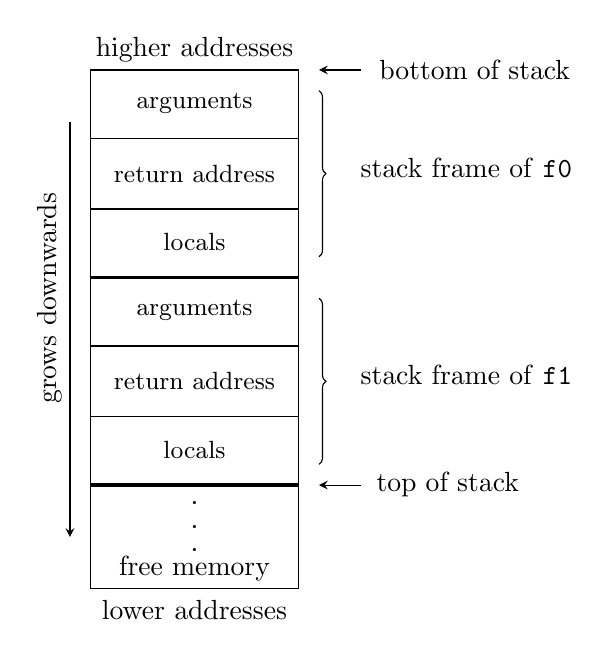
\begin{tikzpicture}[x=0.75pt,y=0.75pt,yscale=-1,xscale=1]

       % Arrow left of stack
       \draw (0,110) node[rotate=90] {grows downwards};
       \draw [-stealth] (10,25) -- (10,225) ;

       % Stack rectangle
       \draw (20,0) -- (120,0) -- (120,250) -- (20,250) -- cycle ;

       % Stack inside
       %% f0
       \draw (70,16) node {\small arguments};
       \draw (20,33) -- (120,33) ;
       \draw (70,50) node {\small return address};
       \draw (20,67) -- (120,67) ;
       \draw (70,83) node {\small locals};

       %% f1
       \draw [very thick] (20,100) -- (120,100) ;
       \draw (70,116) node {\small arguments};
       \draw (20,133) -- (120,133) ;
       \draw (70,150) node {\small return address};
       \draw (20,167) -- (120,167) ;
       \draw (70,183) node {\small locals};

       %% free memory
       \draw [very thick] (20,200) -- (120,200) ;
       \draw (70,220) node[rotate=90] {\large . . . };
       \draw (70,240) node {free memory};

       % Addresses
       \draw (70, -10) node {higher addresses};
       \draw (70, 260) node {lower addresses};

       %% Bottom of stack
       \draw [stealth-] (130,0) -- (150,0) ;
       \draw (205, 0) node {bottom of stack};

       %% Top of stack
       \draw [stealth-] (130,200) -- (150,200) ;
       \draw (192, 200) node {top of stack};

       %% Brace f0
       \draw [decorate, decoration={brace}] (130,10) -- (130,90) ;
       \draw (201,47) node {stack frame of \texttt{f0}};

       %% Brace f1
       \draw [decorate, decoration={brace}] (130,110) -- (130,190) ;
       \draw (201,147) node {stack frame of \texttt{f1}};
   \end{tikzpicture}
   \caption{The layout of the stack when \texttt{f0} has called \texttt{f1}.}
   \label{fig:stack}
\end{figure}

\medskip

Not all data of a program is stored on the stack. Larger and dynamically allocated data is stored in the \emph{heap}. Static and global variables are stored in a separate data segment.


\subsection{Assembly}\label{section:assembly}
Assembly is a low-level programming language in which, generally speaking, each statement corresponds to one instruction executed by the CPU. Assembly statements are compiled into byte sequences of machine code called \emph{opcodes}.

An assembly statement starts with the name of the instruction (the \emph{mnemonic}), followed by its operands (i.e. arguments). \autoref{listing:assembly example} shows an assembly statement where \texttt{mov} is the mnemonic and \texttt{eax} and \texttt{1} are the operands.

\begin{lstlisting}[caption={A single instruction moving the integer \texttt{1} into the register \texttt{eax}.}, label={listing:assembly example}, captionpos=b]
mov eax, 1
\end{lstlisting}

x86 assembly code is written in either Intel syntax (mostly used for Windows development) or AT\&T syntax (mostly used for Linux development). As we focus on Windows in this thesis, we will use the Intel syntax style.

In this section, we will discuss some basic instructions. There are, however, many more instructions used to efficiently perform operations on specific data types.

\subsubsection{Arithmetic Instructions}
x86 provides instructions for basic arithmetic.

\begin{itemize}
    \item \texttt{add op0, op1}: Add the value of \texttt{op1} to \texttt{op0}.
    \item \texttt{sub op0, op1}: Subtract the value of \texttt{op1} from \texttt{op0}.
    \item \texttt{imul op0, op1}: Multiply the value of \texttt{op0} with \texttt{op1} and store the result in \texttt{op0}.
    \item \texttt{idiv op0}: Divide the contents of \texttt{edx:eax} (a 64-bit value of which the 32 most significant bits are taken from \texttt{edx} and the 32 least significant bits are taken from \texttt{eax}) by \texttt{op0} and store the result in \texttt{eax}.
    \item \texttt{inc op0}: Increase the value of \texttt{op0} by 1.
    \item \texttt{dec op0}: Decrease the value of \texttt{op0} by 1.
\end{itemize}

\subsubsection{Logical Instructions}
x86 provides instructions for logical operations.

\begin{itemize}
    \item \texttt{and op0, op1}: Compute the bitwise and \texttt{op0} and \texttt{op1} and store the result in \texttt{op0}.
    \item \texttt{or op0, op1}: Compute the bitwise or of \texttt{op0} and \texttt{op1} and store the result in \texttt{op0}.
    \item \texttt{xor op0, op1}: Compute the bitwise exclusive or of \texttt{op0} and \texttt{op1} and store the result in \texttt{op0}.
    \item \texttt{not op0}: Compute the bitwise not of \texttt{op0} and store the result in \texttt{op0}.
\end{itemize}

\subsubsection{Data Movement Instructions}
x86 provides instructions for moving data between memory and registers.

\begin{itemize}
    \item \texttt{mov op0, op1}: Move the data stored in \texttt{op1} into \texttt{op0}.
    \item \texttt{lea op0, op1}: Move the address (i.e. pointer) stored in \texttt{op1} into \texttt{op0}.
\end{itemize}

\subsubsection{Stack Instructions}
x86 provides instructions for manipulating the call stack.

\begin{itemize}
    \item \texttt{push op0}: Push \texttt{op0} to the stack. This decreases the stack pointer. As pushing data to the stack is essentially writing the data to memory, \texttt{push eax} is equivalent to \autoref{listing:push with mov}.

\begin{lstlisting}[caption={The \texttt{push eax} instruction written in terms of \texttt{sub} and \texttt{mov}.}, captionpos=b, label={listing:push with mov}]
sub esp, 4
mov [esp], eax
\end{lstlisting}

    \item \texttt{pop op0}: Pop the top element from the stack and store it in \texttt{op0}. This increases the stack pointer. \texttt{pop eax} is equivalent to \autoref{listing:pop with mov}.

\begin{lstlisting}[caption={The \texttt{pop eax} instruction written in terms of \texttt{mov} and \texttt{add}.}, captionpos=b, label={listing:pop with mov}]
mov eax, [esp]
add esp, 4
\end{lstlisting}

\end{itemize}

\subsubsection{Control Flow Instructions}\label{section:control flow instructions}
x86 also provides instructions to control the flow of a program. This allows for subroutines (i.e. functions) to be defined and called. It also allows for conditional branching.

\begin{itemize}
    \item \texttt{call op0}: Call a subroutine defined at \texttt{op0}.

    A \texttt{call} performs two operations:
    \begin{enumerate}
        \item It pushes the address after the \texttt{call} instruction to the stack (This is the \emph{return address}).
        \item It changes the \texttt{eip} to the address that is being called (i.e. the next instruction will be at the address that is being called).
    \end{enumerate}

    If \texttt{op0} is an address, the call is \emph{direct}, because the function that is being called is known at compile time or load time. If \texttt{op0} is a register, the call is \emph{indirect} as the address to the function that is called is determined at runtime.

    \item \texttt{ret}: Signal the end of a subroutine and return to the caller. It pops the return address from the stack and jumps to it.
    \item \texttt{jmp op0}: Jump to the instruction at \texttt{op0}.
    \item \texttt{cmp op0, op1} and conditional jumps: It is possible to only jump if a condition is met. The \texttt{cmp} instruction compares the values of its two operands and stores the result in the special \texttt{eflags} register. A conditional jump instruction (e.g. \texttt{je op0}, \texttt{jne op0} and \texttt{jge op0}) reads this result and jumps if its specific condition is met. For example, \texttt{je op0} jumps to \texttt{op0} when the operands of \texttt{cmp} are equal.
\end{itemize}

Because of the control-flow instructions, assembly code is not sequential, but rather a graph structure that can loop and skip code. The code between two control flow instructions is run sequentially and called a \emph{basic block}. This creates a \emph{control flow graph} of basic blocks and paths between these blocks. The conditionals in the code decide which paths are taken. \autoref{fig:control flow graph} shows an example of the control flow graph of a function.

\begin{figure}[ht]
    \centering
    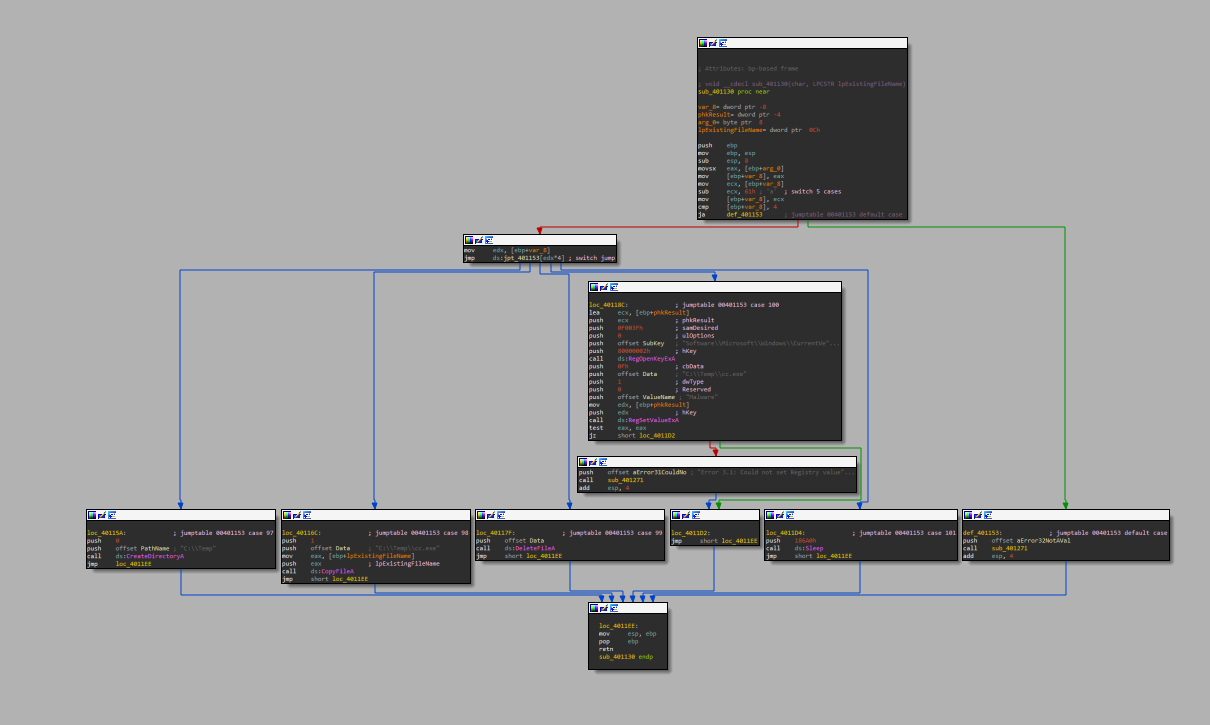
\includegraphics[width=0.9\textwidth]{resources/images/control_flow_graph.png}
    \caption{A screenshot from IDA Pro showing a control flow graph.}\label{fig:control flow graph}
\end{figure}

